% PDP 2027 -- HPCMS special session submission (plan: ../submission2.txt).
% Built on the official IEEEtran v1.8b conference template (bare_conf.tex, CTAN);
% two-column layout as in IEEEtran_HOWTO.pdf. IEEEtran.cls / IEEEtran.bst are
% vendored in this folder, so no system-wide IEEEtran install is needed.
% IEEE conference format, 8 pages max, DOUBLE-BLIND: no author names, affiliations,
% acknowledgements or first-person references to prior work. Cite the authors' earlier
% papers in the third person ("Gilea et al. [x] showed ...").
\documentclass[conference]{IEEEtran}

\usepackage{amsmath,amssymb}
\usepackage{graphicx}
\usepackage{booktabs}
\usepackage{cite}
\usepackage{url}
\usepackage{algorithm}
\usepackage{algpseudocode}
\usepackage[capitalise]{cleveref}

% Hyphenation hints for words LaTeX breaks badly (bare_conf.tex convention).
\hyphenation{op-tical net-works semi-conduc-tor hyper-volume}

% Working title (submission2.txt section 3); final title is written last, once the
% performance results are in. "Parallel" and "Scalability Analysis" are only
% justified if measured speedups make it into the paper -- otherwise retitle.
\title{Parallel Quantum-Inspired Evolutionary Algorithm for Many-Objective
Waste-Collection Routing: Stagnation Diagnosis, Restart Correction, and
Scalability Analysis}

% Double-blind: keep anonymous until camera-ready.
\author{\IEEEauthorblockN{Anonymous Authors}
\IEEEauthorblockA{Affiliation withheld for double-blind review}}

\begin{document}
\maketitle

\begin{abstract}
% TODO: write LAST, after the performance results (submission2.txt section 8).
% Do not reuse the EQTC abstract as-is: it calls all seven instances real-world
% (only the three Sibiu instances are) and claims full ZDT/DTLZ/WFG benchmarking.
\end{abstract}

\begin{IEEEkeywords}
quantum-inspired evolutionary algorithm, many-objective optimization,
capacitated vehicle routing, performance engineering, parallel evaluation
\end{IEEEkeywords}

% Needed only in peer-review mode; a no-op in conference mode (bare_conf.tex).
\IEEEpeerreviewmaketitle

% Page budget (8 pages total) in comments at the top of each section file.
% Budget: ~1.25 pages (intro + related work). DRAFT: the contribution list and the
% last paragraph must be revisited once the performance results exist
% (submission2.txt section 8). Double-blind: the authors' earlier work
% (gilea2026scalable, banciu2025iot) is cited in the third person only.
\section{Introduction}
\label{sec:introduction}

Municipal waste collection is one of the largest recurring logistics costs of a
city, and its routes involve several goals at once: short distances and travel
times, low operating cost, low emissions, and a fair split of work between
crews~\cite{belien2014waste,chen2025smartcities}. Formulated as a capacitated
vehicle routing problem (CVRP) with these goals as separate objectives, it becomes
a \emph{many-objective} problem, for which decomposition- and
reference-vector-based evolutionary algorithms such as MOEA/D~\cite{zhang2007moead}
and RVEA~\cite{cheng2016rvea} are the established tools.

Quantum approaches to multi-objective optimization have so far been
demonstrated on small synthetic binary problems with 3--4
objectives~\cite{kotil2025qamoo,king2025moqa}. Quantum-inspired evolutionary
algorithms (QIEAs)~\cite{han2002qea} borrow the qubit representation but run on
classical hardware, so they can address larger problems today. For the waste-collection routes of Sibiu, Romania~\cite{banciu2025iot}, Gîlea et
al.~\cite{gilea2026scalable} applied a single-objective QIEA to the TSP and found
that it beat a genetic algorithm only on small instances, lost clearly on the
real routes (198--333 collection points), and ran about $3.9\times$ slower. The
authors attributed the loss of diversity at scale to the repair step that
turns measured qubits into valid tours.

To our knowledge, no quantum-inspired method has been evaluated on a real
routing problem with more than three objectives. This paper does so, and asks two
questions that matter for deploying such a method: how good are its solutions
compared with established many-objective algorithms, and where does its runtime
go on a single multicore machine.

We study HQIEA-ARGC, a \emph{Hybrid Quantum-Inspired Evolutionary Algorithm with
Adaptive Rotation-Gate Control}. It is hybrid in that it combines a qubit-angle
encoding with MOEA/D-style decomposition. Its namesake mechanism, ARGC, boosts the
rotation step when population diversity stalls. As we show, ARGC turned out to be
almost inert in practice; the mechanism that actually prevents stagnation is a
plateau-gated restart we added after diagnosing the problem. Our contributions are:
\begin{itemize}
\item A 5-objective waste-collection CVRP model (distance, time, cost,
  load-dependent emissions, workload balance) on real Sibiu road data and
  CVRPLIB instances, with a qubit-angle encoding whose decoding is repair-free
  from qubits to feasible routes.
\item A diagnosis of a hypervolume plateau in HQIEA-ARGC, caused by the ARGC
  stagnation escape almost never firing, and a plateau-gated restart that increases hypervolume by 28--66\%,
  significantly on all seven instances.
\item A comparison with NSGA-II, SPEA2, MOEA/D and RVEA over 30 runs of 500
  generations, which shows that even after this correction HQIEA-ARGC ranks last on
  all seven instances and trails MOEA/D and RVEA by a factor of 1.5--3.3.
\item A runtime profile and Amdahl analysis showing that parallel fitness
  evaluation alone can yield at most 1.4--3.7$\times$, and a parallel design
  informed by it for a hybrid-core CPU.
  % TODO: replace with measured serial + parallel results.
\end{itemize}

\Cref{sec:problem} defines the model, \cref{sec:algorithm} the algorithm, and
\cref{sec:parallel} the runtime profile and parallel design.
\Cref{sec:experiments} reports the experiments and \cref{sec:conclusion}
concludes.

\subsection{Related work}
\emph{Many-objective evolutionary algorithms.} NSGA-II~\cite{deb2002nsga2} and
SPEA2~\cite{zitzler2001spea2} rank solutions by Pareto dominance, which loses
selection pressure as the number of objectives grows. MOEA/D~\cite{zhang2007moead}
decomposes the problem into scalar subproblems defined by weight vectors, and
RVEA~\cite{cheng2016rvea} guides selection with adaptive reference vectors; both
are standard choices for four or more objectives. For routing, permutation
encodings decoded by a split procedure~\cite{prins2004simple} let all of these
algorithms operate on the same search space.

\emph{Quantum and quantum-inspired optimization.} Han and Kim's
QIEA~\cite{han2002qea} represents each gene by a qubit and moves the population
toward good solutions with rotation gates. Later variants target combinatorial
problems such as the TSP~\cite{ma2024qeatsp} and cost-aware workflow scheduling in
hybrid clouds~\cite{hussain2024costaware}. On actual quantum hardware, multi-objective
work has so far used small binary problems~\cite{kotil2025qamoo,king2025moqa}, and
benchmark libraries are only beginning to cover routing~\cite{koch2026qoblib}.
Scalability of the \emph{evaluation}, not only of the search, is a recurring
concern: Ghlib et al.~\cite{ghlib2026scalable} made multi-objective quantum-circuit
synthesis tractable by replacing full-unitary fidelity evaluation with cheaper
block-wise estimates.

\emph{Waste-collection routing.} Beliën et al.~\cite{belien2014waste} survey
operations-research models for waste collection, and Chen et
al.~\cite{chen2025smartcities} identify routing in the waste and transport sectors
as a core multi-objective problem for smart cities. The Sibiu route data used here
was collected by Banciu et al.~\cite{banciu2025iot}.
% TODO: add 1-2 references on parallel metaheuristics / parallel fitness evaluation
% (needed for the PDP audience) once the performance section is written.

% Budget: ~1 page. Source of truth: src/problem.py (objectives, split),
% src/build_instances.py and src/build_cvrplib_instances.py (data generation).
% Every constant below is taken from those files; update both together.
\section{Many-Objective Waste-Collection Routing Model}
\label{sec:problem}

\subsection{Setting}
We model municipal waste collection as a capacitated vehicle routing problem
(CVRP)~\cite{toth2014vrp,belien2014waste}. A directed graph $G=(V,A)$ has
node $0$ as the depot and customers $C=V\setminus\{0\}$, $|C|=n$, each a
collection point with waste demand $q_i>0$. A homogeneous fleet of trucks with
capacity $Q$ starts and ends at the depot. The fleet size is not fixed: the
number of routes $K$ is a consequence of the solution and is itself traded off
through the cost objective. Each arc $(i,j)\in A$ carries a distance $d_{ij}$
(km); the Sibiu matrices are asymmetric, as distances on a real directed
road network generally are.

\subsection{Solution representation and decoding}
Every algorithm in this study searches the same space: a \emph{giant tour}
$\pi$, i.e., a permutation of $C$. A deterministic capacity-first greedy split
walks $\pi$ in order and closes the current route whenever adding the next
customer would exceed $Q$, in the spirit of route-first/cluster-second
decoding~\cite{prins2004simple}. Route $k$ is then the node sequence
$r_k=(0,v_{k,1},\dots,v_{k,m_k},0)$. Because the split never lets a route's
load exceed $Q$, every permutation decodes to a feasible solution: no repair
operator and no penalty term are needed anywhere in the pipeline. This matters
for the qubit encoding (\cref{sec:algorithm}), where an earlier single-objective
QIEA on the same Sibiu routes lost population diversity on large instances
because of its repair step~\cite{gilea2026scalable}.

\subsection{Objectives}
Let $A(r_k)$ be the arcs traversed by route $k$ and $\mathcal{R}=\{r_1,\dots,r_K\}$
the decoded routes. Travel time and variable cost are derived from distance
through a per-arc \emph{road factor} $\rho_{ij}>0$ that models congestion and
road type independently of length:
\begin{equation}
t_{ij}=\frac{\rho_{ij}\,d_{ij}}{\bar v},\qquad c_{ij}=c_v\,\rho_{ij}\,d_{ij},
\end{equation}
with base urban speed $\bar v=25$~km/h and $c_v=1$ cost unit per km. All five
objectives are minimized:
\begin{align}
f_1 &= \sum_{k=1}^{K}\sum_{(i,j)\in A(r_k)} d_{ij}
  && \text{(distance, km)}\\
f_2 &= \sum_{k=1}^{K} T_k,\quad T_k=\sum_{(i,j)\in A(r_k)} t_{ij}
  && \text{(time, h)}\\
f_3 &= c_F\,K+\sum_{k=1}^{K}\sum_{(i,j)\in A(r_k)} c_{ij}
  && \text{(cost)}\\
f_4 &= \sum_{k=1}^{K}\sum_{(i,j)\in A(r_k)}
  \bigl(e_d\,d_{ij}+e_t\,t_{ij}+e_q\,d_{ij}\,L_{k,j}\bigr)
  && \text{(CO$_2$, kg)}\\
f_5 &= \sqrt{\tfrac{1}{K}\textstyle\sum_{k=1}^{K}\bigl(T_k-\bar T\bigr)^2}
  && \text{(workload balance)}
\end{align}
where $c_F=40$ is the fixed cost per vehicle used, $\bar T$ is the mean route
time, and $f_5=0$ when $K=1$. The emission model has a distance term
($e_d=0.7$~kg/km), an idling term that grows with congestion
($e_t=1.2$~kg/h), and a payload term ($e_q=0.004$~kg per km per kg of load).
$L_{k,j}$ is the truck's cumulative load on route $k$ after collecting at
node $j$ (the full route load on the final arc back to the depot). Because a
collection truck fills up as it drives, $f_4$ depends on the \emph{order} of
visits, not only on which arcs are used. $f_3$ couples to fleet size through
$c_F$, and $f_5$ rewards splitting work evenly across trucks, which conflicts
with using few, long routes.

The road factor is essential rather than cosmetic. In an early version of the
model, time, cost and emissions were scalar multiples of distance; the five
objectives were then perfectly correlated and every Pareto front collapsed to a
single point. Drawing $\rho_{ij}$ independently per arc,
$\rho_{ij}\sim\mathrm{LogNormal}(0,\,0.35^2)$, removes this collinearity.

\subsection{Instances}
\Cref{tab:instances} lists the seven instances. The three Sibiu instances use
real road-network distance matrices for waste-collection routes in Sibiu,
Romania, with 333, 198 and 201 collection points. No municipal demand records
are available for these routes, so demands are synthesized as
$q_i\sim\mathcal{U}\{40,\dots,400\}$~kg and capacity is set to
$Q=\lceil 1.15\sum_i q_i/6\rceil$, i.e., about six trucks with 15\% slack. To
test the method beyond one city, we add four CVRPLIB instances~\cite{cvrplib}
(A-n32-k5, A-n33-k5, E-n101-k8, M-n200-k16) with their original demands,
capacities and Euclidean distances. For all seven instances, $\rho_{ij}$ and
therefore $t_{ij}$, $c_{ij}$ and $f_4$ are generated by the same procedure with
a fixed seed, so the objectives are defined identically across data sources.
The synthesized demands and road factors are a modelling assumption, not
measured data; we return to this in \cref{sec:conclusion}.

\begin{table}[t]
\centering
\caption{Benchmark instances. $n$: customers; $\lceil\sum q_i/Q\rceil$: lower
bound on the number of routes.}
\label{tab:instances}
\begin{tabular}{@{}llrrr@{}}
\toprule
Instance & Source & $n$ & $Q$ & $\lceil\sum q_i/Q\rceil$ \\
\midrule
A-n32-k5   & CVRPLIB & 31  & 100    & 5  \\
A-n33-k5   & CVRPLIB & 32  & 100    & 5  \\
E-n101-k8  & CVRPLIB & 100 & 200    & 8  \\
M-n200-k16 & CVRPLIB & 199 & 200    & 16 \\
route2\_199 & Sibiu  & 198 & 8\,469  & 6  \\
route3\_202 & Sibiu  & 201 & 8\,646  & 6  \\
route1\_334 & Sibiu  & 333 & 13\,988 & 6  \\
\bottomrule
\end{tabular}
\end{table}

% Budget: ~1.25 pages. Source of truth: src/qiea.py (module docstring explains every
% mechanism and the logs.txt section that justified it). Constants below match the
% current defaults in QIEA.__init__, _default_theta_bounds, _default_mutation_prob.
\section{HQIEA-ARGC}
\label{sec:algorithm}

HQIEA-ARGC combines a qubit-angle chromosome with MOEA/D-style
decomposition~\cite{zhang2007moead} and two diversity mechanisms: the adaptive
rotation-gate control (ARGC) that gives the algorithm its name, and a
plateau-gated restart that replaced it in practice.
\Cref{alg:hqiea} summarizes one run.

\subsection{Qubit-angle chromosome and repair-free decoding}
Following the quantum-inspired evolutionary algorithm (QIEA) of Han and
Kim~\cite{han2002qea}, each decision variable is a qubit. We restrict it to real
amplitudes, $(\alpha_i,\beta_i)=(\cos\theta_i,\sin\theta_i)$, so the normalization
$\alpha_i^2+\beta_i^2=1$ holds by construction and an individual is simply a vector
$\boldsymbol\theta\in[0,\pi/2]^n$. For routing, the giant tour of
\cref{sec:problem} is obtained by sorting:
\begin{equation}
\pi=\operatorname{argsort}(\boldsymbol\theta).
\end{equation}
Sorting real numbers cannot produce duplicates, so every chromosome is a valid
permutation and no repair is needed. This replaces the binary measurement plus
duplicate-repair pipeline of an earlier QIEA for the same Sibiu routes, in which
Gîlea et al.~\cite{gilea2026scalable} traced the loss of diversity on large
instances to the repair step: as the number of cities grows, most of each tour is
produced by repair rather than by the qubits. Combined with the capacity-first
split, the whole pipeline from qubits to feasible routes is repair-free.

\subsection{Decomposition}
A Das--Dennis simplex lattice~\cite{das1998nbi} with 5 partitions in the
5-objective space gives $H=126$ weight vectors $\mathbf w^1,\dots,\mathbf w^H$.
Each defines a Tchebycheff subproblem
\begin{equation}
g(\mathbf f\mid\mathbf w,\mathbf z^\ast)=\max_{k}\;\max(w_k,10^{-6})\,
\lvert f_k-z^\ast_k\rvert,
\end{equation}
where $\mathbf z^\ast$ is the best value seen so far for each objective. The
population holds one individual per subproblem. The neighborhood $B(i)$ is the
set of $|B(i)|=10$ subproblems whose weight vectors are closest to $\mathbf w^i$.
The same $H=126$ weight vectors are used by the MOEA/D and RVEA baselines, so
these three methods have identical population sizes.

\subsection{Variation operators}
For subproblem $i$, the \emph{guide} is the member of $B(i)$ with the best value
of $g(\cdot\mid\mathbf w^i,\mathbf z^\ast)$, and the \emph{mate} is a random member
of $B(i)$. A child is built in three steps:
\begin{enumerate}
\item \emph{Crossover:} each angle is taken from $\boldsymbol\theta^i$ or from the
  mate with probability $1/2$.
\item \emph{Rotation gate:} each angle moves one step $\Delta\theta$ toward the
  guide, $\theta_j\leftarrow\operatorname{clip}\bigl(\theta_j+\Delta\theta\,
  \operatorname{sgn}(\theta^{\mathrm{guide}}_j-\theta_j),\,0,\,\pi/2\bigr)$.
\item \emph{Qubit flip:} with probability $p_m$ per gene,
  $\theta_j\leftarrow\pi/2-\theta_j$, which swaps $\alpha_j$ and $\beta_j$ (the
  real-amplitude analogue of a Pauli-X gate).
\end{enumerate}
All $H$ children are generated first and then evaluated together as one batch.
Each child then replaces every neighbor $j\in B(i)$ whose current solution it
matches or improves under $g(\cdot\mid\mathbf w^j,\mathbf z^\ast)$. An external
archive keeps all non-dominated solutions found (capped at 500 by random
truncation) and is returned at the end.

\subsection{Size-scaled step and mutation rate}
With the permutation decode, what matters is how far an angle moves relative to
the spacing between neighboring angles, about $\gamma=(\pi/2)/n$. A fixed step
that is fine-grained for $n=31$ becomes a coarse, disruptive move for $n=333$.
The step therefore decays linearly over the run from $\theta_{\max}$ to
$\theta_{\min}$, with
\begin{equation}
\begin{gathered}
\theta_{\min}=\min(0.1,\,2\gamma),\qquad
\theta_{\max}=\min(0.35,\,7\gamma),\\
p_m=\min(0.05,\,1.55/n).
\end{gathered}
\end{equation}
The mutation rate keeps the expected number of flipped genes per child near 1.55
instead of growing with $n$. The caps make all three values reduce exactly to
the constants originally tuned on A-n32-k5 ($n=31$), and shrink them only for
larger instances. In a tuning study on three instances (80-generation runs, 15
seeds), the mutation-rate scaling alone raised the hypervolume by 49\% on
E-n101-k8 and 65\% on route2\_199 (paired Wilcoxon, $p\le0.003$).

\subsection{Adaptive rotation-gate control (ARGC)}
The ARGC mechanism monitors angular diversity,
$D=\frac{1}{Hn}\sum_{i,j}\lvert\theta^i_j-\bar\theta_j\rvert$. If the range of $D$
over the last 10 generations falls below $10^{-3}$, it multiplies the rotation
step by 3 (capped at $\theta_{\max}$) and the mutation rate by 5 for that
generation.

\subsection{Plateau-gated restart}
We found that ARGC almost never fires. In 80-generation runs its trigger was met
in 0 of 400 generations on A-n32-k5 and E-n101-k8, and in 4 of 400 on
route2\_199, because the windowed diversity range bottoms out at about
$2$--$3\times10^{-3}$. Once the population has converged, nothing re-introduces
diversity, and hypervolume freezes (\cref{sec:experiments}). We therefore add a
restart gated on archive growth rather than on angular diversity. When the
archive has not grown for $P=10$ generations, a random half of the $H$
subproblems receive fresh uniform-random angles and are re-evaluated; the other
half keep their solutions, so the restart is elitist. $P$ and the fraction were
chosen on three instances and then confirmed on all seven
(\cref{sec:experiments}).

\begin{algorithm}[t]
\caption{HQIEA-ARGC (one run)}
\label{alg:hqiea}
\small
\begin{algorithmic}[1]
\State $\boldsymbol\theta^{1..H}\sim\mathcal U[0,\pi/2]^n$; evaluate; set
  $\mathbf z^\ast$; archive $\mathcal A\gets$ non-dominated set
\For{$t=1,\dots,G$}
  \State $\Delta\theta,p_m\gets$ linear schedule; apply ARGC boost if $D$ stalled
  \For{$i=1,\dots,H$} \Comment{independent per $i$}
    \State guide, mate $\gets$ from $B(i)$
    \State $\mathbf c^i\gets$ flip(rotate(crossover($\boldsymbol\theta^i$, mate),
      guide, $\Delta\theta$), $p_m$)
  \EndFor
  \State evaluate $\{\mathbf c^i\}_{i=1}^H$ as one batch \Comment{hot spot}
  \State update $\mathbf z^\ast$; neighborhood replacement; update $\mathcal A$
  \If{$\mathcal A$ has not grown for $P$ generations}
    \State reseed $H/2$ random subproblems; evaluate them
  \EndIf
\EndFor
\State \Return $\mathcal A$
\end{algorithmic}
\end{algorithm}

% Budget: ~1 page. Measured part: logs.txt section 17 (src/diag_qiea_profile.py,
% results/diag_qiea_profile*.txt). Framing follows submission2.txt section 8
% ("profiling-guided performance engineering") -- confirm with co-authors.
\section{Runtime Profile and Parallel Design}
\label{sec:parallel}

Before parallelizing anything, we measured where a run spends its time. On a
laptop with an Intel Core i7-12700H and BLAS pinned to one thread, we timed full 500-generation
runs (3 seeds, medians) on a small, a medium and a large instance, and split the
wall-clock time into three parts: fitness evaluation (route split and the five
objectives), archive maintenance, and everything else, i.e., guide selection,
variation operators and neighborhood replacement. We used low-overhead timers for
the shares and a separate cProfile run only to rank functions, since cProfile
inflates pure-Python code.

\begin{table}[t]
\centering
\caption{Runtime breakdown of one HQIEA-ARGC run (500 generations, median of 3
seeds). $S_{\max}$: Amdahl bound on speedup if only evaluation is parallelized.}
\label{tab:profile}
\setlength{\tabcolsep}{3.5pt}
\begin{tabular}{@{}lrrrrrr@{}}
\toprule
Instance & $n$ & Time & Eval. & Archive & Other & $S_{\max}$ \\
\midrule
A-n32-k5    & 31  & 7.7\,s  & 29\% & 2\% & 68\% & 1.4$\times$ \\
route2\_199 & 198 & 16.2\,s & 63\% & 2\% & 35\% & 2.7$\times$ \\
route1\_334 & 333 & 24.2\,s & 73\% & 2\% & 25\% & 3.7$\times$ \\
\bottomrule
\end{tabular}
\end{table}

\Cref{tab:profile} shows the result. Evaluation takes 29--73\% of the runtime and
its share grows with instance size, but each call is cheap: 0.03--0.27\,ms, so a
whole generation's batch of 126 evaluations costs only 4--34\,ms. Archive
maintenance is negligible at about 2\%. The remaining time is almost constant
across instances (5.2--6.0\,s per run) and comes mostly from one source: the
Tchebycheff function is called about 1.9 million times per run (500 generations
$\times$ 126 subproblems $\times$ 10 neighbors $\times$ 3 calls), each time on a
5-element array. The cost is interpreter and library call overhead, not
arithmetic. The restart adds 0--5\% to the runtime, all of it from the extra
evaluations it triggers.

These numbers bound what parallel evaluation alone can achieve. By Amdahl's law,
even with unlimited workers the speedup cannot exceed 1.4$\times$ on the small
instance and 3.7$\times$ on the largest (\cref{tab:profile}). Moreover, the
per-generation batch is small enough that distributing it across processes risks
costing more in communication than it saves. The profile therefore suggests a
different order of work:
\begin{enumerate}
\item \emph{Remove the serial overhead.} Guide selection can compute all
  Tchebycheff values with a single array operation per generation. Replacement is
  sequential, because a neighbor's solution can change within the loop, but the
  child's scores can be computed in advance and the current scores kept in an
  array, which preserves the exact semantics. Evaluation can be compiled with
  Numba.
\item \emph{Parallelize at the right level.} Within one run, evaluation of a batch
  is independent across children, and because all random numbers are drawn in the
  main process, a parallel run with the same seed should produce the same result
  as a serial one; we verify this before timing anything. We compare process-based (multiprocessing) and thread-based (Numba
  \texttt{prange}) parallel evaluation. Across runs, the 1{,}050 independent runs
  of the full study (7 instances $\times$ 5 algorithms $\times$ 30 seeds) are
  embarrassingly parallel.
\item \emph{Account for the hybrid CPU.} The i7-12700H has 6 performance cores
  (12 threads) and 8 efficiency cores. Speedup curves are expected to bend once
  work spills onto the efficiency cores, so we measure performance-core-only,
  efficiency-core-only and mixed placements.
\end{enumerate}

% TODO: results of steps 1-3 go in Sec. experiments (runtime subsection).
% Do NOT state speedups here until measured.

% Budget: ~2.75 pages (1.5 quality + 1.25 performance).
% Numbers in Tables II-III come from results/*_indicators.csv (30 runs x 500 gens,
% restart fix included) and results/tune_qiea_restart_confirm_*.csv (20 seeds).
% Significance: two-sided Mann-Whitney U with Holm correction over the four
% QIEA-vs-baseline comparisons per instance (runs of different algorithms are
% independent, so an unpaired test is used; the paired Wilcoxon used in logs.txt
% gives the same conclusions everywhere).
\section{Experimental Evaluation}
\label{sec:experiments}

\subsection{Setup}
HQIEA-ARGC is compared with NSGA-II~\cite{deb2002nsga2}, SPEA2~\cite{zitzler2001spea2},
MOEA/D~\cite{zhang2007moead} and RVEA~\cite{cheng2016rvea}, all from
pymoo~0.6.2~\cite{blank2020pymoo}. The baselines search the same permutation space
with permutation-valid operators: random-permutation initialization, order
crossover, and inversion mutation. MOEA/D and RVEA use the same $H=126$ weight
vectors as HQIEA-ARGC (MOEA/D with 15 neighbors and neighbor-mating probability
0.9); NSGA-II and SPEA2 use a population of 80. All five algorithms call the same
evaluation function, so they optimize an identical problem. Each algorithm runs
30 times per instance for 500 generations, with seeds $0,\dots,29$. The
population sizes of NSGA-II and SPEA2 (80) differ from the other three (126); in a
separate study that scaled the population of all five algorithms together from
35 to 495, HQIEA-ARGC's relative standing did not change significantly. HQIEA-ARGC
went through the tuning study described in \cref{sec:algorithm}, whereas the
baselines use pymoo's default settings, so any tuning advantage favors
HQIEA-ARGC. The quality runs used Python~3.12, NumPy~2.5.2 and pymoo~0.6.2 on the
machine described in \cref{sec:parallel}.

No true Pareto front is known for these instances, so we measure solution quality
by hypervolume (HV), with spacing and spread as secondary indicators. For each
instance, one reference point, $1.1\times$ the component-wise maximum over all
final fronts of all algorithms and runs, is shared by every run. A Kruskal--Wallis
test checks whether the five algorithms differ on an instance. Each
HQIEA-ARGC--baseline pair is then compared with a two-sided Mann--Whitney $U$ test,
with a Holm correction over the four comparisons per instance.

\subsection{Solution quality}
\Cref{tab:hv} reports each algorithm's mean HV relative to the best algorithm on
that instance. The five algorithms differ significantly on every instance
(Kruskal--Wallis $p<10^{-16}$). No single baseline dominates: SPEA2 and RVEA lead
on the small CVRPLIB instances, and MOEA/D and RVEA on the larger ones and on all
three Sibiu routes. HQIEA-ARGC ranks last on all seven instances, at 30--58\% of
the best algorithm's HV. Of its 28 pairwise comparisons, 27 favor the baseline
significantly. The one exception is route1\_334, the largest instance, where
HQIEA-ARGC reaches 94\% of NSGA-II's HV and the difference is not significant
($p=0.19$). The gap is largest against MOEA/D and RVEA, which reach 1.5 to 3.3
times HQIEA-ARGC's HV on every instance.

HQIEA-ARGC returns 7--25 non-dominated solutions on average, against 53--80
for NSGA-II and SPEA2 and 63--123 for MOEA/D, and has larger spacing values
(106--404 vs.\ 20--75 for NSGA-II and SPEA2). Front size alone does not explain
the HV gap, however: RVEA returns similarly small fronts (16--23 solutions) and
still achieves the best HV on four instances.

\begin{table}[t]
\centering
\caption{Mean hypervolume relative to the best algorithm per instance (1.000 =
best; 30 runs, 500 generations; HQIEA = HQIEA-ARGC). $^\dagger$: HQIEA-ARGC vs.\ NSGA-II not
significant ($p=0.19$); all other HQIEA-ARGC comparisons $p<0.01$ (Mann--Whitney,
Holm).}
\label{tab:hv}
\setlength{\tabcolsep}{4pt}
\begin{tabular}{@{}lrrrrr@{}}
\toprule
Instance & HQIEA & NSGA-II & SPEA2 & MOEA/D & RVEA \\
\midrule
A-n32-k5    & 0.571 & 0.989 & 0.992 & 0.876 & \textbf{1.000} \\
A-n33-k5    & 0.541 & 0.956 & \textbf{1.000} & 0.840 & 0.994 \\
E-n101-k8   & 0.300 & 0.478 & 0.542 & 0.978 & \textbf{1.000} \\
M-n200-k16  & 0.330 & 0.368 & 0.429 & \textbf{1.000} & 0.928 \\
route2\_199 & 0.581 & 0.748 & 0.815 & 0.987 & \textbf{1.000} \\
route3\_202 & 0.489 & 0.660 & 0.720 & 0.902 & \textbf{1.000} \\
route1\_334 & 0.577$^\dagger$ & 0.614 & 0.691 & \textbf{1.000} & 0.927 \\
\bottomrule
\end{tabular}
\end{table}

\subsection{Diagnosis: plateau and restart correction}
Before the restart was added, HQIEA-ARGC's HV was only 17--45\% of the best
algorithm's on every instance. To see why, we traced HV every 10 generations for
all algorithms, with and without the restart, on a small, a medium and a large
instance (3 seeds each, reference point fixed per run; \cref{fig:trace}).
Without the restart, HQIEA-ARGC is competitive with the baselines for the first
50--100 generations on A-n32-k5, but on all three instances its HV eventually
stops improving (no gain above 0.5\% of its final value) from generation 60--150
on A-n32-k5 and 410--450 on route2\_199, while every baseline keeps improving
until generation 500. On route1\_334 the plateau had not yet been reached at
generation 500, but progress had slowed. The ARGC trigger, meant for exactly this
situation, stays inactive (\cref{sec:algorithm}). With the restart, HQIEA-ARGC
continues to improve until the end of the run on all three instances, and its
final HV is 16--68\% higher than without it on the same seed.

\begin{figure*}[t]
\centering
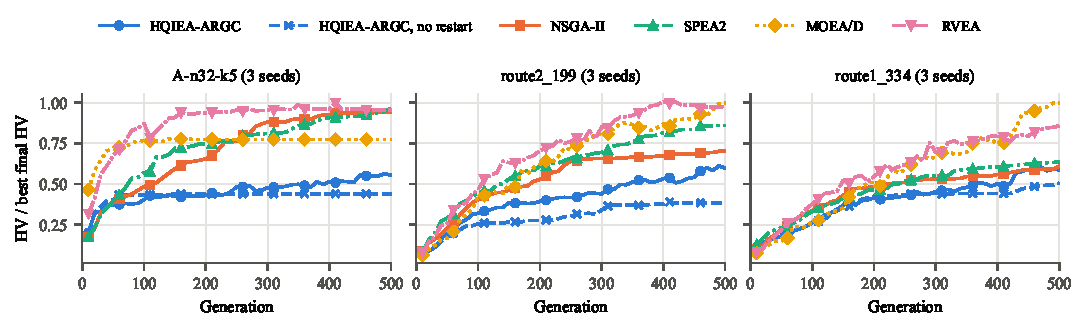
\includegraphics[width=\textwidth]{figures/trace_restart.pdf}
\caption{Hypervolume vs.\ generation, relative to the best final HV of any
algorithm in the same run (median over 3 seeds). Without the restart (dashed),
HQIEA-ARGC stops improving early on A-n32-k5 and late on route2\_199; with the
restart (solid) it keeps improving, but stays below the baselines.}
\label{fig:trace}
\end{figure*}

\Cref{tab:restart} isolates the restart's effect. With seeds matched, so that both
variants start from the same initial population, the restart increases HV
significantly on all seven instances, by 28--66\%. It is the only change in our
tuning study that was significant on every instance in the same direction. It
narrows HQIEA-ARGC's gap to the best algorithm by roughly half, from 17--45\% to
30--58\% of the best HV, but does not close it.

\begin{table}[t]
\centering
\caption{Effect of the plateau-gated restart: HQIEA-ARGC mean HV with vs.\
without restart (20 seeds, 500 generations, paired Wilcoxon on matched seeds).}
\label{tab:restart}
\begin{tabular}{@{}lrr@{}}
\toprule
Instance & HV change & $p$ \\
\midrule
A-n32-k5    & $+29.7\%$ & $3.7\times10^{-3}$ \\
A-n33-k5    & $+32.0\%$ & $1.3\times10^{-4}$ \\
E-n101-k8   & $+66.0\%$ & $1.9\times10^{-6}$ \\
M-n200-k16  & $+35.4\%$ & $2.6\times10^{-4}$ \\
route2\_199 & $+36.1\%$ & $6.3\times10^{-5}$ \\
route3\_202 & $+40.4\%$ & $1.9\times10^{-6}$ \\
route1\_334 & $+27.7\%$ & $2.1\times10^{-4}$ \\
\bottomrule
\end{tabular}
\end{table}

Several other levers did not explain the remaining gap. Tuning the neighborhood
size $|B(i)|$, making ARGC fire more often, changing its boost magnitude, and scaling
the population size $H$ jointly for all five algorithms (35 to 495) either had no
significant effect or made HV worse. Promising 5-seed screens repeatedly failed
15-seed confirmation, so we changed a default only after a confirmation run.

\subsection{Runtime and parallel performance}
% TODO: depends on the performance work (submission2.txt sections 7-8).
% (The runtime-breakdown table is already in Sec. parallel, tab:profile.)
% - Serial optimization results (vectorized Tchebycheff, Numba evaluator).
% - Speedup/efficiency vs workers, multiprocessing vs Numba threads, P/E cores.
% - Time-to-quality: HV vs wall-clock for all five algorithms.
% Hardware: Intel Core i7-12700H (6 P-cores + 8 E-cores, 20 threads), 62 GiB,
% Python 3.12, NumPy 2.5.2, pymoo 0.6.2, BLAS pinned to 1 thread per process.

% Budget: ~0.75 pages. DRAFT: revisit once the performance results exist.
\section{Discussion, Limitations and Conclusion}
\label{sec:conclusion}

\emph{What the results show.} A qubit-angle encoding with argsort decoding and a
capacity-first split gives a repair-free pipeline for many-objective routing, and
it produces valid, non-degenerate fronts on all seven instances. The most
consistent effect we found was not a parameter setting but a mechanism failure
and its correction: the stagnation-escape trigger almost never fired, the
population stalled, and a restart gated on archive growth increased hypervolume by
28--66\% on every instance. Even so, HQIEA-ARGC ranks last on all seven
instances. Scaling the step size and mutation rate with instance size improved
it but did not close the gap to MOEA/D and RVEA, and the neighborhood size, ARGC
settings and population size had no significant effect.

\emph{A structural hypothesis.} Since every hyperparameter lever we tested
failed, the remaining difference is more likely structural, for example in how
solutions are varied, selected and replaced. It is not simply front size: RVEA
returns fronts as small as HQIEA-ARGC's and still leads on four instances. One
candidate stands out: all four baselines vary solutions with operators designed
for permutations (order crossover and inversion), whereas HQIEA-ARGC changes
tours only indirectly, by moving angles that are then sorted. It is the only
algorithm without permutation-specific operators, and the only one that ranks
last everywhere. Among the baselines, the selection scheme then separates
MOEA/D and RVEA from NSGA-II and SPEA2 on the larger instances. Testing this, for
example by adding a permutation operator to HQIEA-ARGC, is future work.

\emph{Limitations.} Demands on the Sibiu routes and the road factors on all
instances are synthesized with a fixed seed, because no measured bin-fill or
congestion data is available; results should be read as relative comparisons
under a documented model, not as operational savings. The emission term charges
each arc with the load collected up to and including its destination node. The
study runs on a single laptop CPU with hybrid cores; multi-node and GPU
execution are not evaluated.
% TODO: add the performance conclusions here once measured.

\emph{Conclusion.} We evaluated a quantum-inspired evolutionary algorithm on a
real 5-objective waste-collection routing problem. The plateau-gated restart is a
large, reproducible improvement, but the algorithm does not match MOEA/D and RVEA,
and the runtime profile shows that parallelizing its fitness evaluation alone
would give little. Future work will test the structural hypothesis above, and
move the evaluation to multi-node and GPU platforms.


% Double-blind: leave acknowledgements out until the camera-ready version.
% \section*{Acknowledgment}
% The authors would like to thank ...

\bibliographystyle{IEEEtran}
\bibliography{refs}

\end{document}
